\documentclass[journal]{IEEEtran}
\usepackage[a5paper, margin=10mm, onecolumn]{geometry}
\usepackage{lmodern}

\setlength{\headheight}{1cm}
\setlength{\headsep}{0mm}

\usepackage{gvv-book}
\usepackage{gvv}
\usepackage{cite}
\usepackage{amsmath,amssymb,amsfonts,amsthm}
\usepackage{graphicx}
\graphicspath{{./figs/}}
\usepackage{xcolor}
\usepackage{txfonts}
\usepackage{enumitem}
\usepackage{mathtools}
\usepackage{hyperref}
\usepackage{tikz}
\usepackage{tkz-euclide}

\begin{document}

\bibliographystyle{IEEEtran}
\vspace{3cm}

\title{2.10.65}
\author{EE25BTECH11036 - M Chanakya Srinivas}
\maketitle

\renewcommand{\thetable}{\theenumi}
\setlength{\intextsep}{10pt}
\renewcommand\theequation{\arabic{equation}}





\section*{Problem Statement}
Let \(OACB\) be a parallelogram with \(O\) at the origin and \(OC\) a diagonal. Let \(D\) be the midpoint of \(OA\). Using vector methods, prove that \(BD\) and \(CO\) intersect in the same ratio. Determine this ratio.

\section*{Solution}

\subsection*{Step 1: Define position vectors of vertices}
\begin{align}
\vec{O} &= \myvec{0\\0}, \\
\vec{A} &= \vec{a}, \\
\vec{C} &= \vec{c}, \\
\vec{B} &= \vec{A} + \vec{C}.
\end{align}

Midpoint \(D\) of \(OA\):
\begin{align}
\vec{D} &= \frac{\vec{O} + \vec{A}}{2} = \frac{1}{2} \vec{A}.
\end{align}

\subsection*{Step 2: Represent lines in vector form}

Line \(BD\):
\begin{align}
\vec{R_1} &= \vec{B} + \lambda (\vec{D} - \vec{B}) \\
&= \vec{B} + \lambda \left(\frac{1}{2}\vec{A} - (\vec{A} + \vec{C})\right) \\
&= \vec{B} - \lambda \left(\frac{1}{2}\vec{A} + \vec{C}\right)
\end{align}

Line \(CO\):
\begin{align}
\vec{R_2} &= \vec{C} + \mu (\vec{O} - \vec{C}) \\
&= \vec{C} - \mu \vec{C} = (1-\mu)\vec{C}
\end{align}

\subsection*{Step 3: Intersection condition}

\[
\vec{R_1} = \vec{R_2} \quad \Rightarrow \quad 
\vec{B} - \lambda \left(\frac{1}{2}\vec{A} + \vec{C}\right) = (1-\mu)\vec{C}
\]

Substitute \(\vec{B} = \vec{A} + \vec{C}\):
\begin{align}
\vec{A} + \vec{C} - \lambda \left(\frac{1}{2}\vec{A} + \vec{C}\right) = (1-\mu)\vec{C}
\end{align}

\subsection*{Step 4: Equate coefficients of \(\vec{A}\) and \(\vec{C}\)}
\begin{align}
\text{Coefficient of } \vec{A}: & \quad 1 - \frac{\lambda}{2} = 0 \quad \Rightarrow \quad \lambda = 2 \\
\text{Coefficient of } \vec{C}: & \quad 1 - \lambda = 1 - \mu \quad \Rightarrow \quad \mu = 2
\end{align}

\subsection*{Step 5: Interpret the ratio}

- On \(BD\), \(\lambda = 2\) implies the intersection divides \(BD\) in ratio \(2:1\).  
- On \(CO\), \(\mu = 2\) implies the intersection divides \(CO\) in ratio \(2:1\).  

\begin{align}
\boxed{\text{The lines $BD$ and $CO$ intersect in the ratio } 2:1.}
\end{align}






\begin{figure}[h]
    \centering
    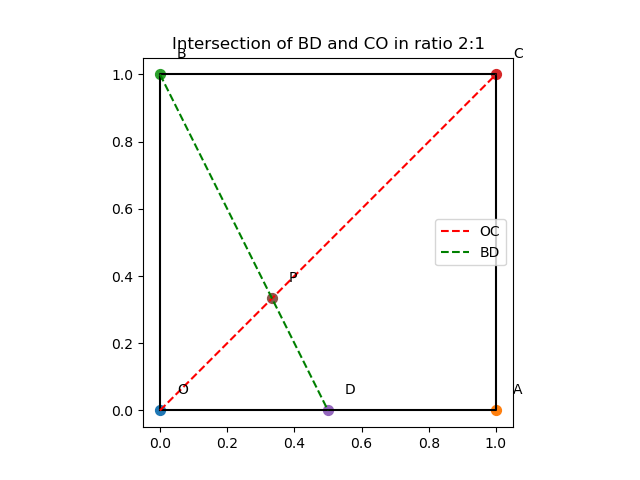
\includegraphics[width=0.9\columnwidth]{figs/fig51.png}
    \caption{}
    \label{fig:placeholder}
\end{figure}

\begin{figure}
    \centering
    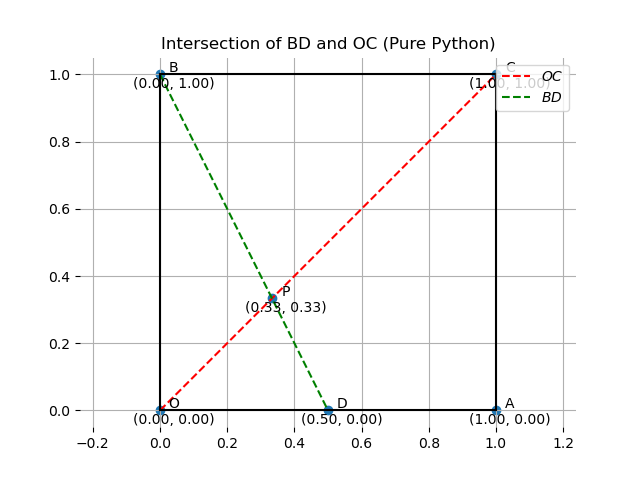
\includegraphics[width=0.9\columnwidth]{figs/fig52.png}
    \caption{}
    \label{fig:placeholder}
\end{figure}
\end{document}